\documentclass[11pt]{article}
\usepackage[T1]{fontenc}
\usepackage{graphicx}
\usepackage{wrapfig}
\usepackage{titling}
\usepackage[bottom=10mm]{geometry}
\usepackage{graphicx} % Required for inserting images
\usepackage[htt]{hyphenat}
\usepackage{hyperref}
\usepackage{amsfonts}

\graphicspath{{./images/}}
%\setlength{\droptitle}{-5em}

\title{B1 Numerical Algorithms: Computing value of $\pi$}
\author{Jin Rhee}
\date{4 November 2024}

\begin{document}
\maketitle

\thispagestyle{empty}
\paragraph{Introduction} This report discusses three different methods to estimate the value of $\pi$ and details of their respective implementation and error.
Code was developed in C++17 on Apple M1 arm64. Code: \url{https://github.com/JinRhee/b1-numerical-algorithms-practical}
\paragraph{Method and Implementation}
Three methods are used to calculate an estimate of $
\pi$:
    
\par{Monte Carlo.}
This method is implemented by picking $N$ pairs $(x,y)$ of random numbers (from independent uniform real distributions),
and returning the ratio $\frac{N'}{N}\times 4$ where $N'$ is the number of pairs that satisfy $x^2+y^2 \leq 1$.
Multiple number of samples are tested $N=2^{k},\ k\in[0, 25]$ with relative error and error bar considerations.
\par{Newton-Raphson.}
This root-finding algorithm is applied to $f(x) = \sin(x)$ which has the roots $x=n\pi,\ n\in \mathbb{Z}$. The implementation
iterates $x_n=x_{n-1}+\tan{x_{n-1}}$ and terminates when $|x_n - x_{n-1}| \leq \epsilon$ (i.e. at convergence criteria), returning $x_n$.
Multiple error values are tested (default $\epsilon=0.1$) and the algorithm is given an initial estimate of $x_0=2$.
\par{Chudnovsky algorithm.}
This algorithm \ref{eq:chudnovsky} is proposed as the third method to estimate $\pi$. In short, this algorithm calculates
$\pi$ as the sum of an infinite series.

\paragraph{Error}
All three methods are implemented in 8-byte \texttt{double} which offers a maximum precision to
16 decimal points.
\par{Monte Carlo.} The Central Limit Theorem states that the sample average approaches the normal distribution as
the sample size increases. We can thus use the sample variance to plot error bars representing
a standard deviation. A \texttt{double} constant value of $\pi$ is used to calculate the relative error, which is
plotted against the sample size \ref{fig:monte_carlo_plot}.
\par{Newton-Raphson.} An analysis using the Taylor expansion shows that the error propogates quadratically $\epsilon_{n+1}\propto \epsilon_n^2$
at each iteration. The quadratic error propogation can be used with the initial error to quantify error at some iteration: $\epsilon_{n} \propto \epsilon_{0}^{2^{n-1}}$
\par{Chudnovsky algorithm.} Error originates from the truncation of the infinite series and the precision of the floating point 
representation of the \texttt{double} data type. The later is dominant, as empirically the series sum of more than 2 terms
returns the same value.

\paragraph{Discussion} The Chudnovsky algorithm is most efficient and accurate method out of the three. Though requiring 
factorial calculation, it only needs to sum two terms of the series to achieve
higher accuracy than that of Newton-Raphson or Monte Carlo.
\par Empirically, $[\texttt{Chud., Newt., Mont.}]$
take $[\texttt{0.00025ms, 0.00063ms, 1551.81ms}]$ to produce errors of: $[\texttt{2.93-14, 5.00e-08, 3.92e-04}]$.
Due to both superior accuracy and efficiency, the Chudnovsky algorithm is recommended for estimating $\pi$.
\newpage
\section*{Appendix}
\subsection*{Figures}
\begin{figure}[h!]
    \centering
    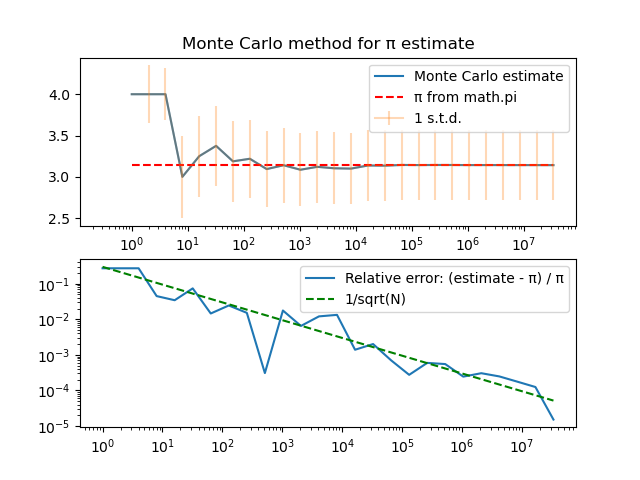
\includegraphics[width=\textwidth]{monte_carlo_plot.png}
    \caption{Monte Carlo method error plots.}
    \label{fig:monte_carlo_plot}
\end{figure}
\subsection*{Equations}
\begin{equation}
    \label{eq:chudnovsky}
    \frac{1}{\pi} =  12\sum_{k=0}^{\infty}\frac{a}{b} \frac{(-1)^k(6k)!(545140134k+13591409)}{(3k)!(k!)^3(640320)^{3k+3/2}}
\end{equation}
\end{document}


%refs
%https://en.cppreference.com/w/cpp/numeric/random/uniform_real_distribution
%https://en.cppreference.com/w/cpp/numeric/math/tan
%https://en.wikipedia.org/wiki/Chudnovsky_algorithm#Python_code
%https://en.wikipedia.org/wiki/Monte_Carlo_integration
%https://math.libretexts.org/Bookshelves/Calculus/CLP-1_Differential_Calculus_(Feldman_Rechnitzer_and_Yeager)/06%3A_Appendix/6.03%3A_C-_Root_Finding/6.3.02%3A_C.2_The_Error_Behaviour_of_Newton%27s_Method
